
\documentclass[11pt]{article}

%% WRY has commented out some unused packages %%
%% If needed, activate these by uncommenting
\usepackage{geometry}                % See geometry.pdf to learn the layout options. There are lots.
%\geometry{letterpaper}                   % ... or a4paper or a5paper or ...
\geometry{a4paper,left=2.5cm,right=2.5cm,top=2.5cm,bottom=2.5cm}
%\geometry{landscape}                % Activate for rotated page geometry
%\usepackage[parfill]{parskip}    % Activate to begin paragraphs with an empty line rather than an indent

\usepackage{natbib}

%for figures
%\usepackage{graphicx}

\usepackage{color}
\definecolor{mygreen}{RGB}{28,172,0} % color values Red, Green, Blue
\definecolor{mylilas}{RGB}{170,55,241}
%% for graphics this one is also OK:
\usepackage{epsfig}

%% AMS mathsymbols are enabled with
\usepackage{amssymb,amsmath}

%% more options in enumerate
\usepackage{enumerate}
%\usepackage{enumitem}

%% insert code
\usepackage{listings}

\usepackage[utf8]{inputenc}

\usepackage{hyperref}

%\newcommand{\backslash}{\char`\\}

\usepackage{soul}

\title{Rough notes on the Brazil Current System in the ECCO2 hierarchy}
\date{}
\author{CBR\thanks{Scripps Institution of Oceanography, University
        of California, San Diego; \texttt{crocha@ucsd.edu}}\,\,\,\,\& MMM}
\begin{document}

\maketitle
\vspace{-1cm}

\newcommand{\com}{\, ,}
\newcommand{\per}{\, .}

%% Averages
% Use \bar to over line solo symbols

\newcommand{\av}[1]{\bar{#1}}
\newcommand{\avbg}[1]{\overline{#1}}
\newcommand{\avbgg}[1]{\overline{#1}}

% A nice definition
\newcommand{\defn}{\ensuremath{\stackrel{\mathrm{def}}{=}}}

% space in equations
\newcommand{\qqand}{\qquad \text{and} \qquad}
\newcommand{\qand}{\quad \text{and} \quad}

% equations
\def\beq{\begin{equation}}
\def\eeq{\end{equation}}

\def\bea{\begin{align}}
\def\ena{\end{align}}

% calculus
\newcommand{\ord}{\mathcal{O}}
\newcommand{\p}{\partial}
\newcommand{\ii}{{\rm i}}
\newcommand{\dd}{{\rm d}}
\newcommand{\id}{{\, \rm d}}
\newcommand{\ee}{{\rm e}}
\newcommand{\DD}{{\rm D}}
\newcommand{\wavy}{\text{wavy}}
\newcommand{\qg}{\text{qg}}
\newcommand{\dt}{\Delta t}
\newcommand{\dx}{\Delta x}
\newcommand{\be}{\beta}

\newcommand{\al}{\alpha}
\newcommand{\bx}{\boldsymbol{x}}
\newcommand{\by}{\boldsymbol{y}}
\newcommand{\bu}{\boldsymbol{u}}
\newcommand{\bv}{\boldsymbol{v}}


\newcommand{\half}{\tfrac{1}{2}}
\newcommand{\halfrho}{\tfrac{1}{2}}
\newcommand{\rz}{{}}
\newcommand{\bn}{\boldsymbol{\hat n}}
\newcommand{\br}{\boldsymbol{r}}
\newcommand{\bR}{\boldsymbol{R}}
\newcommand{\bA}{\ensuremath {\boldsymbol {A}}}
\newcommand{\bB}{\ensuremath {\boldsymbol {B}}}
\newcommand{\bU}{\ensuremath {\boldsymbol {U}}}
\newcommand{\bE}{\ensuremath {\boldsymbol {E}}}
\newcommand{\bN}{\ensuremath {\boldsymbol {\mathrm{N}}}}
\newcommand{\bJ}{\ensuremath {\boldsymbol {J}}}
\newcommand{\bXX}{\ensuremath {\boldsymbol {\mathcal{X}}}}
\newcommand{\bFF}{\ensuremath {\boldsymbol {F}}}
\newcommand{\bF}{\ensuremath {\boldsymbol {F}^{\sharp}}}
\newcommand{\bG}{\ensuremath {\boldsymbol G}}
\newcommand{\bSigma}{\ensuremath {\boldsymbol {\Sigma}}}
\newcommand{\bvarphi}{\ensuremath {\boldsymbol {\varphi}}}
\newcommand{\bxi}{\ensuremath {\boldsymbol {\xi}}}
\newcommand{\avbxi}{\overline{\ensuremath {\boldsymbol {\xi}}}}

% math cal

\newcommand{\J}{\mathcal{J}}
\newcommand{\K}{\mathcal{K}}
\newcommand{\cG}{\mathcal{G}}
\newcommand{\cF}{\mathcal{F}}
\newcommand{\cN}{\mathcal{N}}
\newcommand{\cL}{\mathcal{L}}
\newcommand{\cS}{\mathcal{S}}
\newcommand{\cE}{\mathcal{E}}


% san serif for matrices and differential operators
%\newcommand{\helmn}{\mathsf{H}_n}
\newcommand{\helmm}{\triangle_m}
\newcommand{\helmn}{\triangle_n}
\newcommand{\helms}{\triangle_s}
\newcommand{\helm}{\triangle}
\newcommand{\sA}{\mathsf{A}}
\newcommand{\sB}{\mathsf{B}}
\newcommand{\sG}{\mathsf{G}}
\newcommand{\sI}{\mathsf{I}}
\newcommand{\sJ}{\mathsf{J}}
\newcommand{\gsJ}{\breve{\mathsf{J}}}
\newcommand{\sU}{\mathsf{U}}
\newcommand{\sP}{\mathsf{P}}
\newcommand{\sQ}{\mathsf{Q}}
\newcommand{\sR}{\mathsf{R}}
\newcommand{\sL}{\mathsf{L}}
\newcommand{\Lu}{\mathsf{L}(\what{u}_k)}
\newcommand{\Nu}{\mathsf{N}(\what{u}_k)}
\renewcommand{\L}{\mathsf{L}}
\newcommand{\N}{\mathsf{N}}
\newcommand{\sH}{\mathsf{H}}
\renewcommand{\sJ}{\mathsf{J}}
\renewcommand{\sI}{\mathsf{I}}
\renewcommand{\L}{\mathsf{L}}
\newcommand{\sM}{\mathsf{M}}
\newcommand{\sT}{\mathsf{T}}
\newcommand{\sGamma}{\mathsf{\Gamma}}
\newcommand{\sOmega}{\mathsf{\Omega}}
\newcommand{\sSigma}{\mathsf{\Omega}}
\newcommand{\sbeta}{\mathsf{\beta}}
\newcommand{\sPi}{\mathsf{\Pi}}
\newcommand{\sC}{\mathsf{C}}
\newcommand{\sQy}{\mathsf{Q}}
\renewcommand{\sb}{\mathsf{b}}

% u
\newcommand{\uhat}{\what{u}_k}

% angle brackets

\def\la{\langle}
\def\ra{\rangle}
\def\laa{\left \langle}
\def\raa{\right \rangle}


%grads and div's
\newcommand{\bcdot}{\hspace{-0.1em} \boldsymbol{\cdot} \hspace{-0.12em}}
\newcommand{\bnabla}{\boldsymbol{\nabla}}
\newcommand{\bnablaH}{\bnabla_{\! \mathrm{h}}}
\newcommand{\grad}{\bnabla}
\newcommand{\gradH}{\bnablaH}
\newcommand{\curl}{\bnabla \!\times\!}
\newcommand{\diver}{\bnabla \bcdot }
\newcommand{\cross}{\times}
\newcommand{\lap}{\nabla^2}


%varthetas and thetas
\newcommand{\vth}{\vartheta}
\newcommand{\psii}{\psi^{\mathrm{i}}}
\newcommand{\thb}{\theta^{\mathrm{-}}}
\newcommand{\vthb}{\vartheta^{\mathrm{-}}}
\newcommand{\vthbhat}{{\hat{\vartheta}}^{\mathrm{-}}}
\newcommand{\vThb}{\varTheta^{\mathrm{-}}}
\newcommand{\psib}{\psi^{\mathrm{-}}}
\newcommand{\tht}{\theta^{\mathrm{+}}}
\newcommand{\vtht}{\vartheta^{\mathrm{+}}}
\newcommand{\vththat}{{\hat{\vartheta}}^{\mathrm{+}}}
\newcommand{\vthtbhat}{{\hat{\vartheta}}^{\pm}}
\newcommand{\vTht}{\varTheta^{\mathrm{+}}}
\newcommand{\vthtb}{\vartheta^{\pm}}
\newcommand{\vThtb}{\varTheta^{\pm}}

% nondimensional numbers
\renewcommand{\Re}{\mathrm{Re}}
\newcommand{\Ro}{\mathrm{Ro}}
\newcommand{\Ri}{\mathrm{Ri}}

%psi's
%Galerking coefficient for psi:
\newcommand{\gpsi}{\breve \psi}
\newcommand{\gpsic}{{\breve \psi}^\star}
\newcommand{\gtau}{\breve \tau}
\newcommand{\gtauc}{{\breve \tau}^\star}
\newcommand{\gphi}{\breve \phi}
\newcommand{\gq}{\breve q}
\newcommand{\gU}{\breve U}
\newcommand{\gQ}{\breve Q}
\newcommand{\gsigma}{\breve \sigma}


\newcommand{\psit}{\psi^{\mathrm{+}}}
\newcommand{\psithat}{{\hat{\psi}}^{\mathrm{+}}}
\newcommand{\psibhat}{{\hat{\psi}}^{\mathrm{-}}}
\newcommand{\psitb}{\psi^{\pm}}
\newcommand{\psitbhat}{{\hat{\psi}}^\pm}
\newcommand{\St}{S^{\mathrm{+}}}
\newcommand{\Sb}{S^{\mathrm{-}}}
\newcommand{\phb}{\phi^{\mathrm{-}}}
\newcommand{\pht}{\phi^{\mathrm{+}}}
\newcommand{\tautb}{\tau^{\pm}}
\newcommand{\sigmatb}{\sigma^{\pm}}


\newcommand{\bur}{\left(\tfrac{f_0}{N}\right)^2}
\newcommand{\ibur}{\left(\tfrac{N}{f_0}\right)^2}
\newcommand{\Nm}{N_{\mathrm{mix}}}
\newcommand{\xim}{\xi_{\mathrm{mix}}}
\newcommand{\hs}{h_*}
\renewcommand{\sp}{\mathsf{p}}
\newcommand{\se}{\mathsf{e}}
\newcommand{\sptb}{\mathsf{p}^\pm}


%nmax is a problem:
%\newcommand{\nmax}{n_{\mathrm{max}}}
\newcommand{\nmax}{\mathrm{N}}
\newcommand{\mmax}{\mathrm{M}}

\newcommand{\WKB}{\mathrm{WKB}}
\newcommand{\Lam}{\Lambda}
\newcommand{\tha}{\theta}
\newcommand{\kap}{\kappa}
\newcommand{\bphi}{\boldsymbol{\phi}}
\newcommand{\third}{\tfrac{1}{3}}
\newcommand{\cs}{c^\star}
\newcommand{\dstar}{{\star\star}}
\newcommand{\nt}{n^{\mathrm{trnc}}}
\newcommand{\sDp}{\mathsf{D}^1_{\nmax}}
\newcommand{\sDpp}{\mathsf{D}^2_{\nmax}}
\newcommand{\sD}{\mathsf{D}}
\newcommand{\sDN}{\mathsf{D_\nmax}}
\newcommand{\sK}{\mathsf{K_2}}
\newcommand{\stheta}{\mathsf{\theta}}
\newcommand{\sphi}{\mathsf{\phi}}
\newcommand{\sq}{\mathsf{q}}
\newcommand{\cosech}{\text{csch}\,}
\newcommand{\sinc}{\text{sinc}\,}

%%%%%%%%% %%%%
\newcommand{\zp}{z^+}
\newcommand{\zm}{z^-}
\newcommand{\qA}{q^A_{\nmax}}
\newcommand{\psiB}{\psi^B_{\nmax}}
\newcommand{\phiB}{\phi^B_{\nmax}}
\newcommand{\eye}{\boldsymbol{\hat{i}}}
\newcommand{\jay}{\boldsymbol{\hat{j}}}
\newcommand{\kay}{\boldsymbol{\hat{k}}}
\newcommand{\psiG}{\psi^{\mathrm{G}}}
\newcommand{\qG}{q^{\mathrm{G}}}
\newcommand{\uG}{u^{\mathrm{G}}}
\newcommand{\UG}{U^{\mathrm{G}}}
\newcommand{\UGN}{U^{\mathrm{G}}_{\nmax}}
\newcommand{\QGN}{Q^{\mathrm{G}}_{\nmax}}
\newcommand{\sumoddn}{\sum_{n = 1, n~ \text{odd}}^{\nmax}}

% bretherton 
\newcommand{\qBr}{q_{\mathrm{Br}}}
\newcommand{\psiBr}{\psi_{\mathrm{Br}}}

\newcommand{\ep}{\epsilon}


\section{Introduction}

How well does a state-of-art state estimate represents the Brazil Current (BC) System
off southeast Brazil? An accurate answer to that question seems impossible
today given that a characterization of the BC System is notably limited.
To date most of what is known about that western boundary current system derives
from few quasi-synoptic hydrographic and velocity observations and ever fewer
current meter arrays \cite[and references therein]{rocha_etal2014}. There are a
few well-known characteristics of the BC System off Brazil that provide a testbed
for state-estimates. In particular, the presence of an Intermediate Western Boundary
Current (IWBC) over the continental north of $\sim\!\!25^\circ$ and the downstream thickening of the BC
are trademarks of the BC System off southeast Brazil \citep{rocha_etal2014}.
Both the formation of the IWBC and the thickening of the BC are associated with
the rather parochially named ``Santos Bifurcation'' (the bifurcation of the
subtropical gyre at intermediate levels).

In these notes we analyze two outputs of the ECCO2 hierarchy: ECCOv4 and
ECCOv4-LLC2160 \citep{forget_etal2015}. The base solution ECCOv4 consists of a 22-year synthesis (1992+)
of millions of observations using a general circulation model; the interpolated
resolution of the output is 1/2$^\circ$. The ECCOv4-LLC2160 is a 1/24$^\circ$
forward solution spun up from the ECCOv4 state-estimate. The LLC2160 output is
available for 2 years starting  March 2011. Figure \ref{LLC2160currents} shows
LLC2160 2-year time-average of surface and 800 m currents in the domain region.
At the surface, the BC dominates the circulation over most of the continental
slope and outer shelf; the currents largely follow the isobaths. At 800 m,
the flow of the southward BC is depicted following south of 25.5$^\circ$, whereas
a the northward IWBC flows north of  25$^\circ$ over the continental slope; eastward of
the IWBC there is a weak southward flow. The latter is not apparent in the 22-year average
ECCOv4 data and may not survive a longer averaging.

\begin{figure}[!ht]
  \label{LLC2160currents}
  \centering
      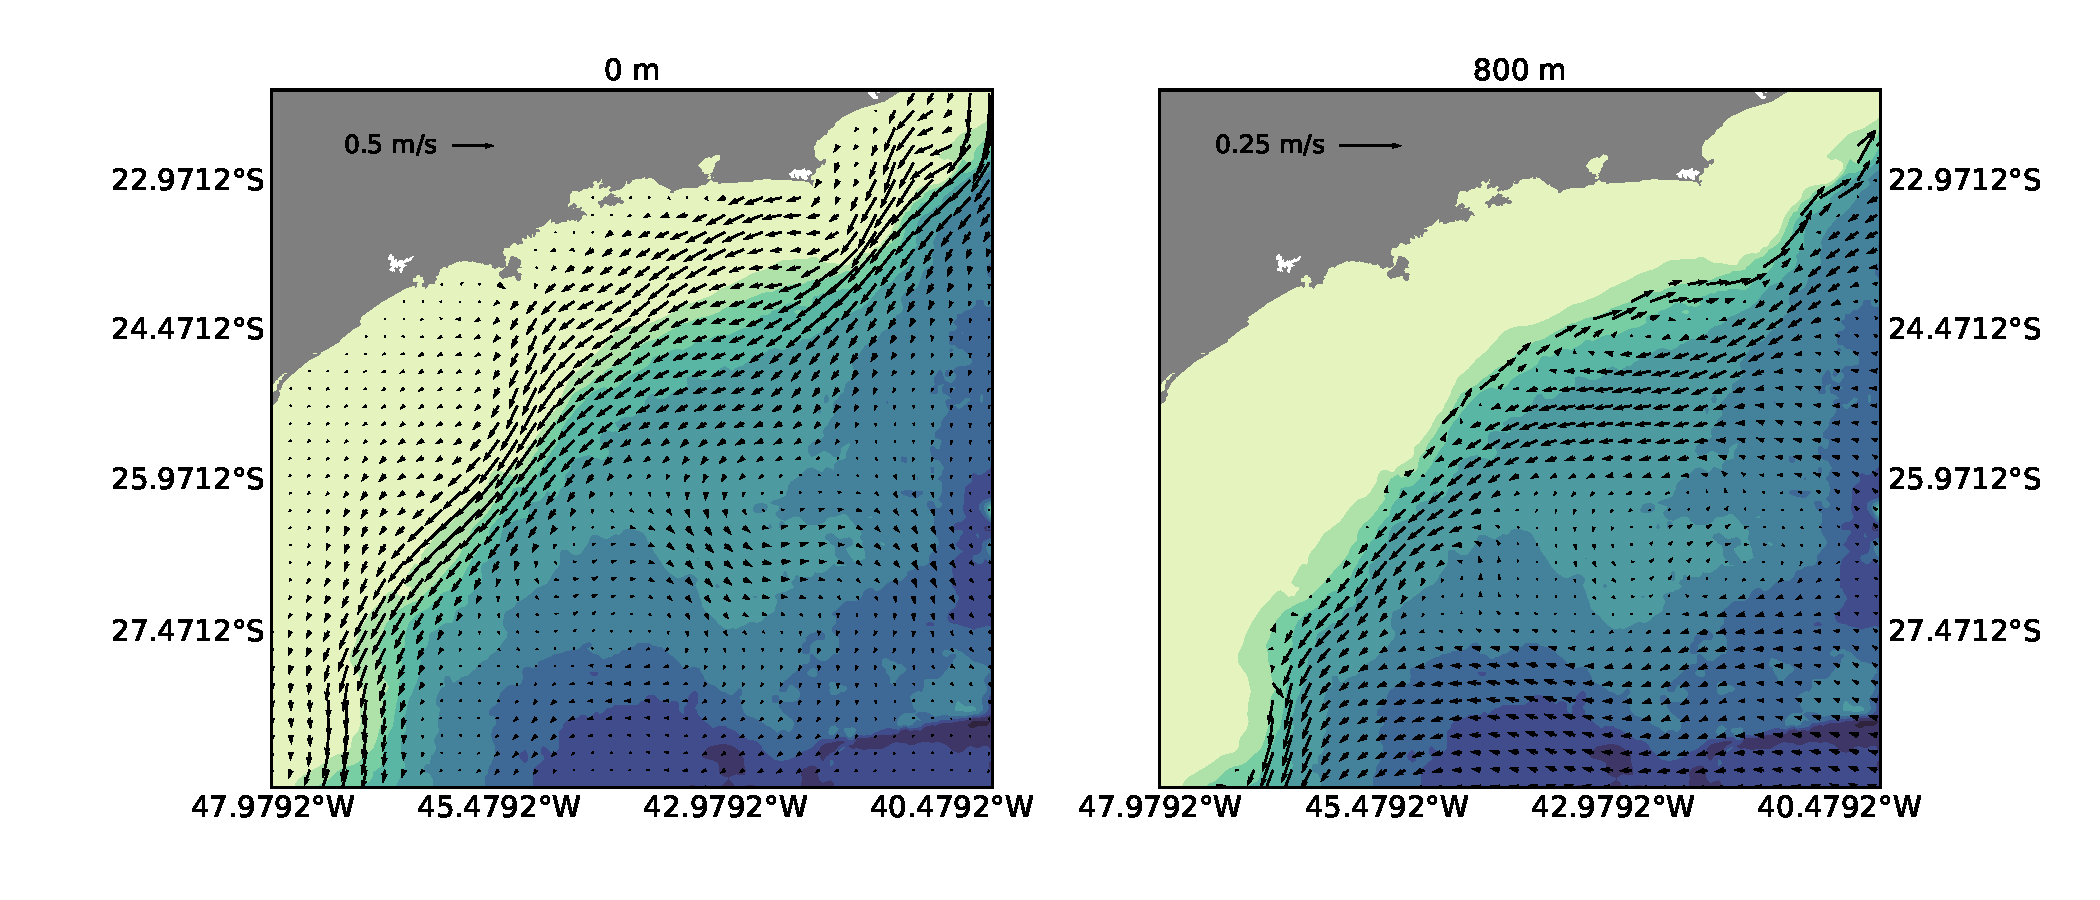
\includegraphics[width=1.05\textwidth]{figs/LLC2160_currents.pdf}
  \caption{Horizontal velocity at the surface and 800 m from the LLC2140
            ECCO2 simulation.}
\end{figure}

\section{Does the ECOOv4 and LLC2160 represent the BC thickening?}
The ECCOv4 appears to represent the BC thickening rather satisfactorily.
In particular, figure \ref{ECCOv4Sec} shows two 2-year time-averaged velocity
sections off Cabo Frio and Santos. The BC vertical extent and magnitude of
horizontal velocity are consistent with observations \citep[e.g., ][]{rocha_etal2014}.
The BC thickening is clearly depicted in a along-stream section of along-stream
velocity (Figure \ref{ECCOv4Thick}). Consistent with the results of
\cite{rocha_etal2014}, most
of the thickening of the BC occurs south of $25^\circ$.

Not surprisingly, the structure IWBC is not well represented in the coarse-resolution
ECCOv4 output (the thin jet is replaced by a broad sluggish intermediate flow),
though its transport may be well captured. The much finer resolution of the
LLC2160 simulation, however, does allow for the representation of the IWBC jet
(Figure \ref{LLC2160Sec}). The outer shelf/upper continental slope LLC2160 off
Cabo Frio is consistent with the classic BC-IWBC picture depicted by observations
\citep{silveira_etal2004}. Because Santos is located at approximately the latitude
of formation of the IWBC, the intermediate flow over the upper slope is notably weak.


(It may also be crucial for the representation of the IWBC jet the
use of a partial-cell formulation
to properly account for the flow near topography. Need to think harder about this.)


\begin{figure}[!ht]
\label{ECCOv4Sec}
  \centering
      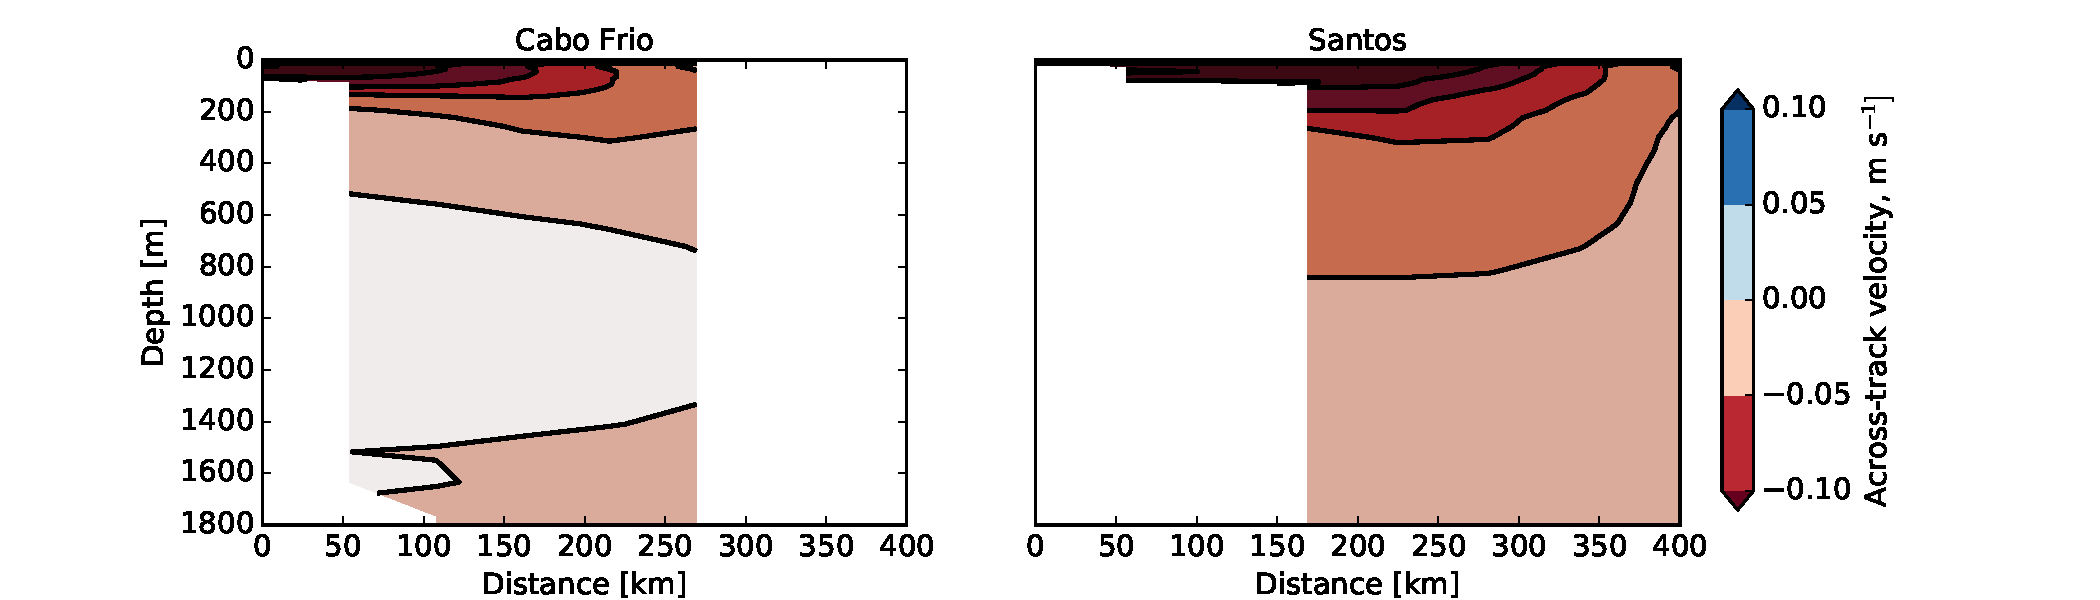
\includegraphics[width=1.05\textwidth]{figs/ECCOv4_VelSections.pdf}
  \caption{ECCOv4 vertical sections of velocity across-track off Cabo Frio (left)
          and Santos (right).}
\end{figure}

\begin{figure}[!ht]
  \centering
      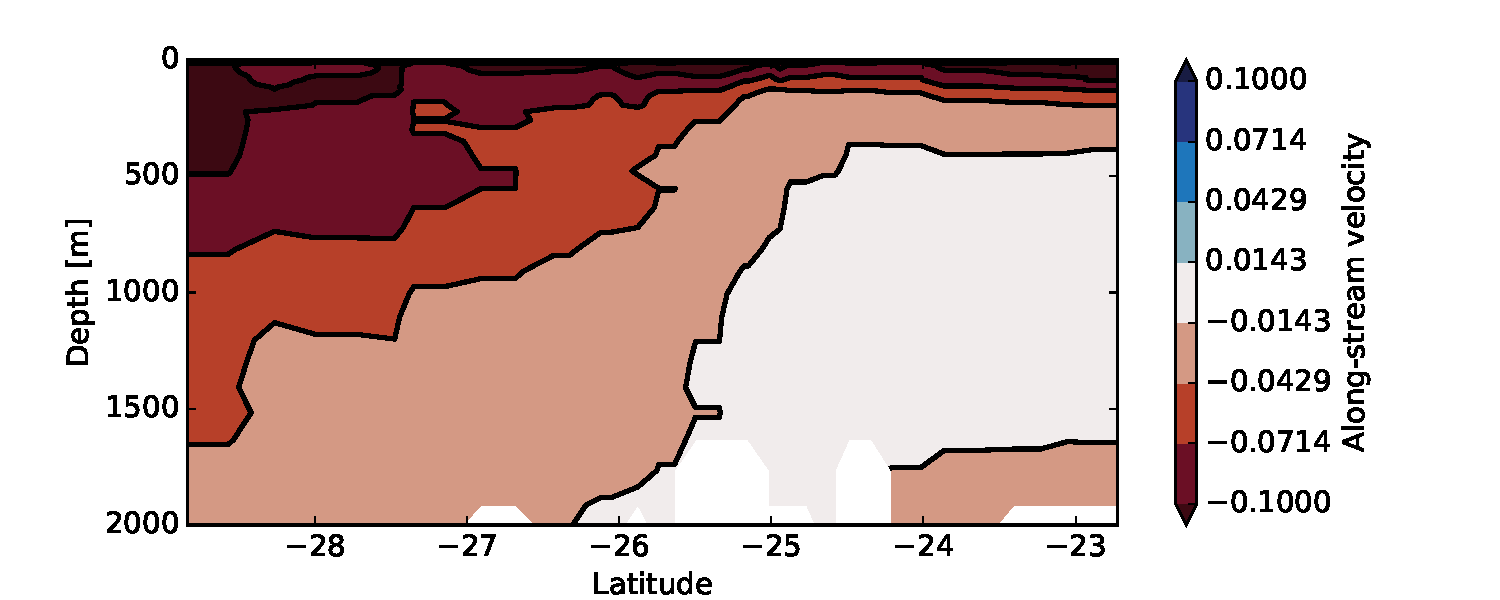
\includegraphics[width=1.05\textwidth]{figs/ECCOv4_AlonTrackVel.pdf}
  \caption{ECCOv4: vertical sections of approximate along-stream velocity along
          the 1750 isobath.}
          \label{ECCOv4Thick}
\end{figure}

\begin{figure}[!ht]
  \centering
      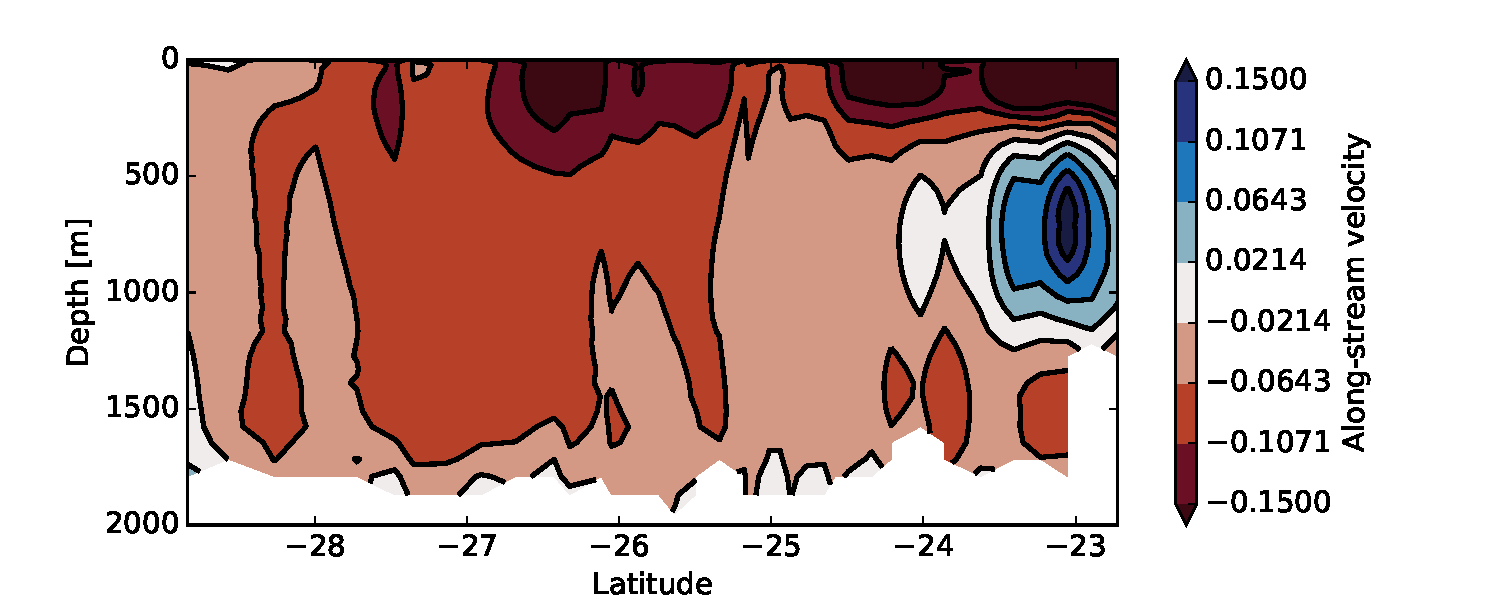
\includegraphics[width=1.05\textwidth]{figs/LLC2160_AlonTrackVel.pdf}
  \caption{LLC2160: vertical sections of approximate along-stream velocity along
          the 1750 isobath.}
          \label{LLC2160Thick}
\end{figure}

\begin{figure}[!ht]
  \centering
      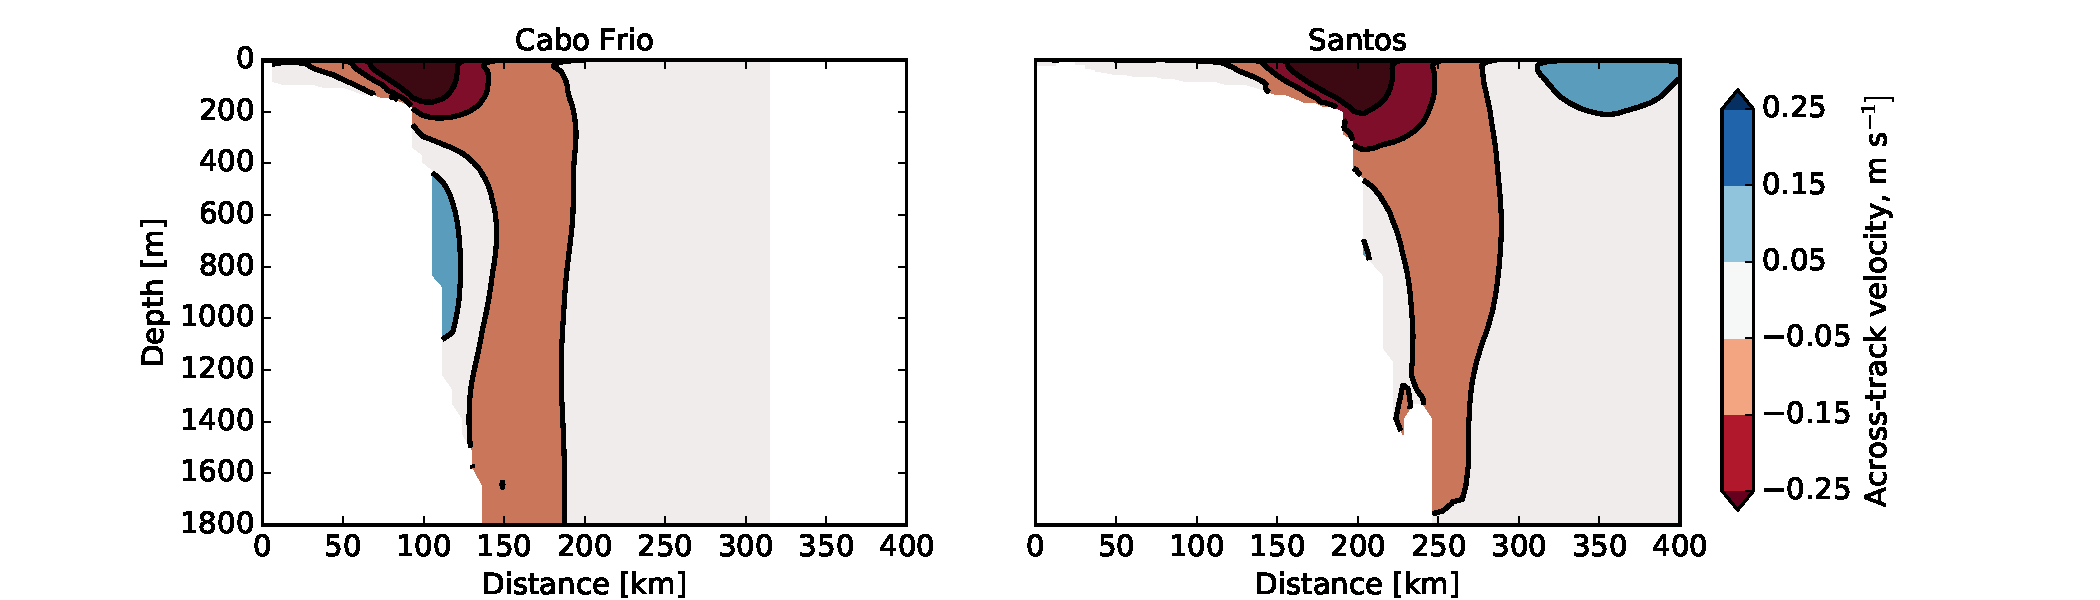
\includegraphics[width=1.05\textwidth]{figs/LLC2160_VelSections.pdf}
  \caption{LLC2160 vertical sections of velocity across-track off Cabo Frio (left)
          and Santos (right).}
          \label{LLC2160Sec}
\end{figure}

%\begin{figure}[!ht]
%\label{LLC2160Thick}
%  \centering
%      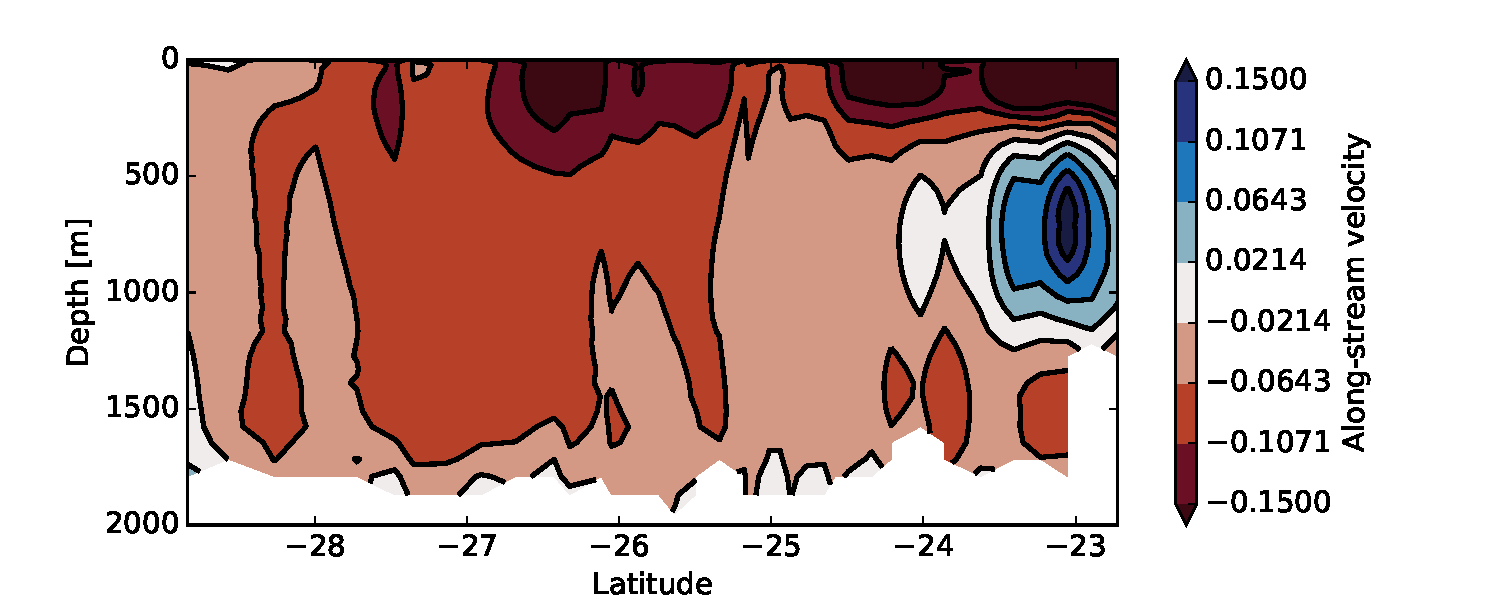
\includegraphics[width=1.05\textwidth]{figs/LLC2160_AlonTrackVel.pdf}
%  \caption{LLC2160: vertical sections of approximate along-stream velocity along
%          the 1750 isobath.}
%\end{figure}

\section{The Brazil Current System off Sao Sebastiao}
The BC System circulation off Sao Sebastiao is something
intermediate between Cabo Frio and Santos (Figue \ref{LLC2160_SaoSeba}).
The Brazil Current occupied the upper 400 m, spanning the outer shelf and
part of the upper slope. The IWBC is well formed, but it is not as strong as off Cabo Frio.


\begin{figure}[!ht]
  \centering
      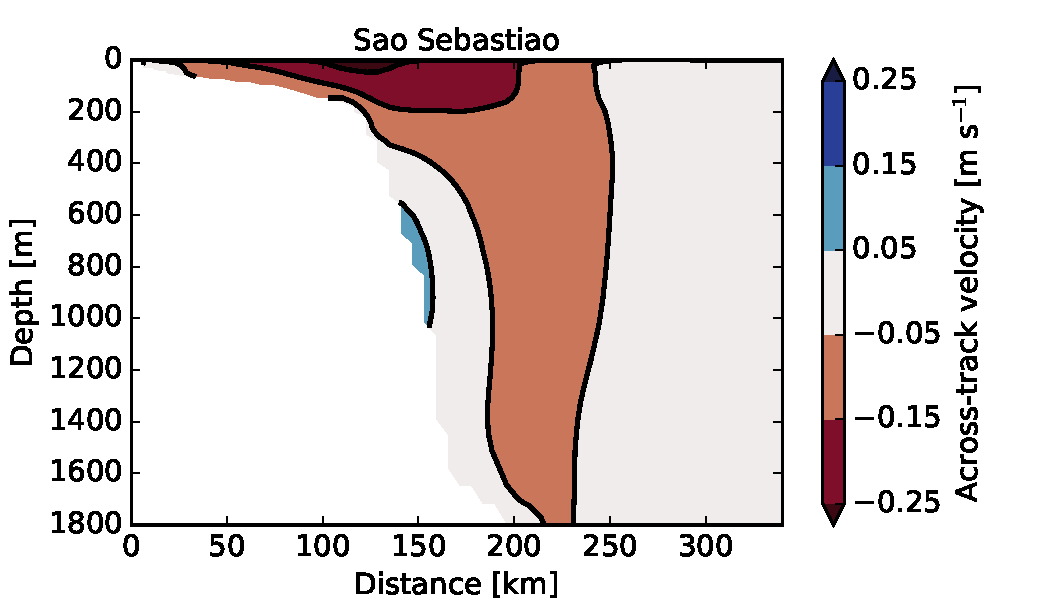
\includegraphics[width=.6\textwidth]{figs/LLC2160_VelSection_SaoSeba.pdf}
  \caption{LLC2160 vertical section of velocity across-track off Sao Sebastiao.}
          \label{LLC2160_SaoSeba}
\end{figure}

\section{Time-averaged current near the bottom}
Figue \ref{LLC2160_bottom} shows near-bottom current from 2-year time-averaged
LLC2160 output.

\begin{figure}[!ht]
  \centering
      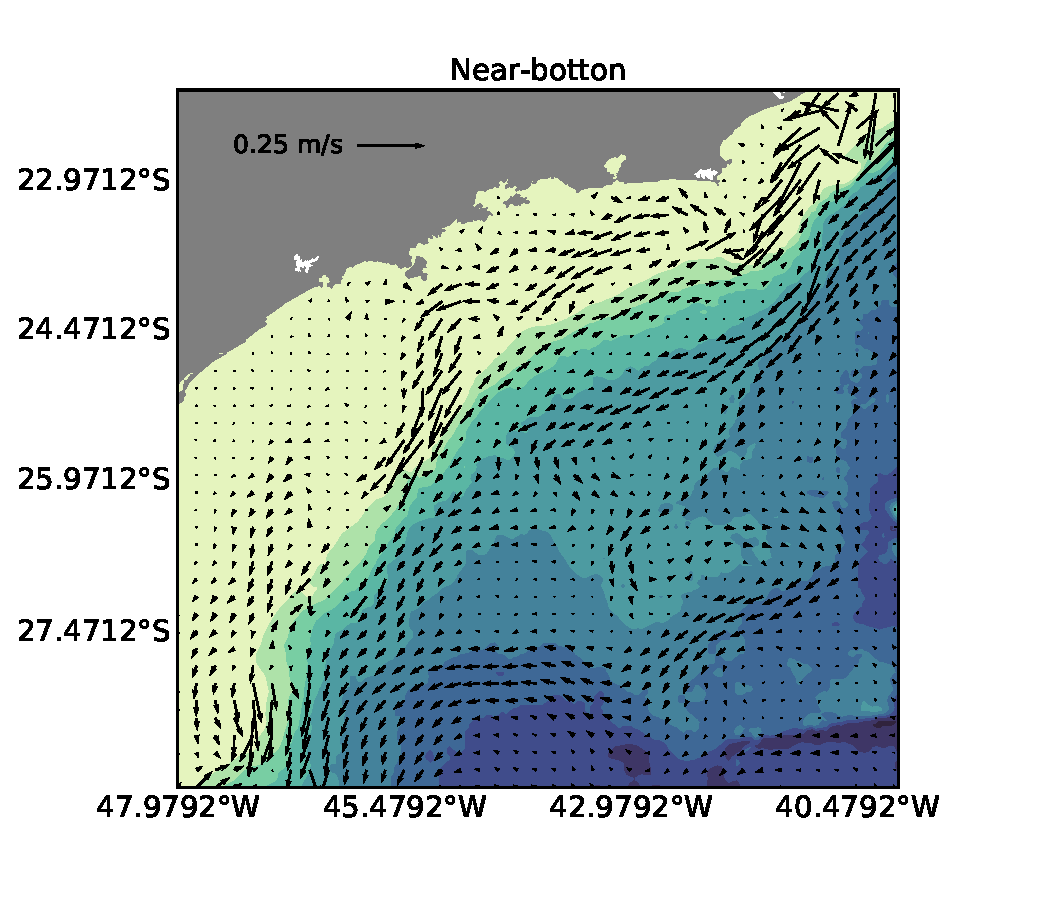
\includegraphics[width=.8\textwidth]{figs/LLC2160_bottom-currents.pdf}
  \caption{LLC2160 time-averaged near-bottom current off southeast Brazil.}
          \label{LLC2160_bottom}
\end{figure}

\clearpage
\bibliographystyle{chicago}
\bibliography{BCECCO.bib}

\end{document}
